\section{il teorema di Lagrange e criteri di monotonia}

\begin{theorem}[Fermat]
\mymark{***}
Sia $f\colon (a,b)\to \RR$ una funzione derivabile.
Se $x_0\in (a,b)$ è un punto di massimo o minimo per $f$ allora
$f'(x_0)=0$.
\end{theorem}
%
\begin{proof}
\mymark{***}
Senza perdere di generalità possiamo suppore che $x_0$ sia un punto di massimo per $f$.
Sappiamo che
\[
  f'(x_0) = \lim_{x\to x_0}\frac{f(x)-f(x_0)}{x-x_0}.
\]
Visto che $x_0$ è un punto dell'intervallo aperto $(a,b)$ la funzione $f$ è definita in un intorno destro di $x_0$ e quindi possiamo restingere il limite ai valori $x>x_0$ ottenendo:
\[
  f'(x_0) = \lim_{x\to x_0^+}\frac{f(x) - f(x_0)}{x-x_0}.
\]
Visto che $x_0$ è un punto di massimo per $f$ sappiamo che $f(x)-f(x_0)\le 0$. Essendo $x-x_0>0$ l'intero rapporto incrementale risulta essere non positivo.
Dunque, per il teorema della permanenza del segno,
possiamo concludere che $f'(x_0)\le 0$.

Ma possiamo anche restringere la funzione ad un intorno sinistro di $x_0$ e osservare che
\[
  f'(x_0) = \lim_{x\to x_0^-}\frac{f(x)-f(x_0)}{x-x_0}.
\]
Ma ora il numeratore è, come prima, non positivo mentre il denominatore $x-x_0$ è negativo. Dunque il rapporto incrementale stavolta è non negativo e quindi, per la permanenza del segno, $f'(x_0) \ge 0$.

Abbiamo scoperto quindi che $f'(x_0)\le 0$ e $f'(x_0)\ge 0$
da cui deduciamo $f'(x_0)=0$.
\end{proof}

Il teorema di Fermat si può
enunciare dicendo che ogni punto di massimo o minimo relativo interno
al dominio di una funzione in cui la funzione è derivabile
è necessariamente un punto critico.
In particolare per determinare massimi e minimi assoluti e relativi
di una funzione sarà sufficiente esaminare i punti di frontiera,
i punti di non derivabilità e i punti critici.

\begin{exercise}[derivazione della legge di Snell dal principio di Fermat]
  \label{ex:snell}
  \index{legge!di Snell}%
  \index{Snell!legge di}%
  \index{principio!di Fermat}%
  \index{Fermat!principio di}%
Vogliamo quantificare la legge di rifrazione della luce secondo 
cui un raggio luminoso genera un punto angoloso nel punto in cui 
il raggio attraversa la superficie di separazione 
tra due mezzi con indici di rifrazione diversi. 
Ad esempio un raggio che attraversa una lente di vetro passa prima dall'aria 
al vetro e poi dal vetro all'aria.
In questi passaggi il raggio viene deviato, permettendo di fatto di 
utilizzare le lenti per focalizzare la luce.

\begin{figure}
  \begin{center}
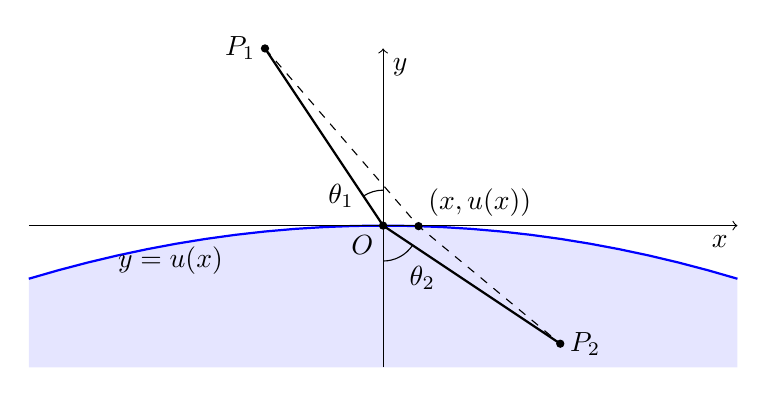
\begin{tikzpicture}[scale=1.5]
    % Surface (parabolic for illustration)
    \fill[blue!10] (-3,-1.2) -- (3,-1.2) -- plot[domain=3:-3] (\x, {-0.05*\x*\x}) -- cycle;
    \draw[thick, blue, domain=-3:3] plot (\x, {-0.05*\x*\x});
    \node at (-1.8,-0.3) { \( y = u(x) \) };

    % Axes
    \draw[->] (-3,0) -- (3,0) node[below left]{$x$};
    \draw[->] (0,-1.2) -- (0,1.5) node[below right]{$y$};
    
    
    % Point O
    \fill (0,0) circle (1pt) node[below left]{$O$};
    
    % Incident ray
    \draw[thick] (-1,1.5) -- (0,0);
    \fill (-1,1.5) circle (1pt) node[left]{$P_1$};
    
    % Refracted ray
    \draw[thick] (0,0) -- (1.5,-1);
    \fill (1.5,-1) circle (1pt) node[right]{$P_2$};
    
    % Variation ray
    \draw[dashed] (-1,1.5) -- (0.3,{-0.05*0.3*0.3}) -- (1.5,-1);
    \fill (0.3,{-0.05*0.3*0.3}) circle (1pt) node[above right]{$(x,u(x))$};

    % angles
    \draw (0,0.3) arc (90:123.69:0.3) node[left]{$\theta_1$};
    \draw (0,-0.3) arc (-90:-33.69:0.3) node[midway, below right]{$\theta_2$};
\end{tikzpicture}  \end{center}
\caption{Principio di Fermat, vedi esercizio~\ref{ex:snell} sulla derivazione della legge di Snell.}
\end{figure}

\mynote{
  Questo principio è noto come principio di Fermat 
  ed è la prima formulazione del principio di minima azione in fisica.
  Nella fisica moderna si sostituisce la richiesta di punto di minimo con quella di punto stazionario
  prendendo quindi la tesi del teorema di Fermat come assioma fondamentale 
  invece che l'ipotesi.
  }%
Si ipotizza che tra due punti sufficientemente vicini lungo il percorso 
del raggio luminoso la luce percorra il tragitto che minimizza il tempo di percorrenza.
Si ipotizza inoltre che la velocità della luce sia costante all'interno di ciascun mezzo
(ma diversa nei due mezzi).

Consideriamo il punto $O$ in cui la luce passa da un mezzo all'altro
e consideriamo il piano contenente i due raggi incidenti e rifratti nel 
punto $O$. Su questo piano mettiamo un sistema di assi cartesiani 
con la $x$ orientata lungo il piano tangente in $O$ alla superificie 
di separazione tra i due mezzi e con l'asse $y$ perpendicolare 
a tale superficie. 
Siano $(x_1,y_1)$ e $(x_2,y_2)$ le coordinate di due punti qualunque $P_1$ e $P_2$, 
il primo sul raggio di incidenza e il secondo sul raggio rifratto, diversi da $O$
e sufficientemente vicini ad $O$ per poter ipotizzare che il percorso 
più breve da $P_1$ a $P_2$ sia quello che percorre prima il segmento 
da $P_1$ a $O$ e poi il segmento da $O$ a $P_2$.

L'angolo di incidenza $\theta_1$ e l'angolo di rifrazione $\theta_2$
sono quindi dati dalle seguenti formule:
\[
  \sin \theta_1 = -\frac{x_1}{\sqrt{x_1^2+y_1^2}},\qquad
  \sin \theta_2 = \frac{x_2}{\sqrt{x_2^2+y_2^2}}.
\]

Sia $u(x)$ la funzione che descrive il profilo della superificie 
di separazione tra i due mezzi. Per come abbiamo scelto il sistema di 
coordinate sia ha $u(0)=0$ e $u'(0)=0$. 
%Supponiamo che $u$ sia di classe $C^1$.
Possiamo allora scrivere la funzione $f(x)$ che rappresenta
il tempo di percorrenza di un raggio luminoso che percorre 
il segmento da $(x_1,y_1)$ a $(x,u(x))$ nel primo mezzo e poi 
il segmento da $(x,u(x))$ a $(x_2,y_2)$ nel secondo mezzo.
Se $c_1$ e $c_2$ sono le velocità della luce nei due mezzi 
si avrà:
\[
  f(x) = \frac{1}{c_1} \sqrt{(x - x_1)^2 + (u(x) - y_1)^2} +
         \frac{1}{c_2} \sqrt{(x - x_2)^2 + (u(x) - y_2)^2}.
\]
Per ipotesi la funzione $f$ assume un minimo in $x=0$ 
e dunque, per il teorema di Fermat, si deve avere $f'(0)=0$.
Calcoliamo quindi la derivata di $f$ 
\[
  f'(x) = \frac{1}{c_1}\frac{x - x_1 + (u(x)-y_1)u'(x)}{\sqrt{(x-x_1)^2 + (u(x)-y_1)^2}} +
          \frac{1}{c_2}\frac{x - x_2 + (u(x)-y_2)u'(x)}{\sqrt{(x-x_2)^2 + (u(x)-y_2)^2}}
\]
e la valutiamo in $x=0$, 
ricordando che $u(0)=0$ e $u'(0)=0$:
\[
  f'(0) = \frac{1}{c_1}\frac{- x_1}{\sqrt{x_1^2 + y_1^2}} +
          \frac{1}{c_2}\frac{- x_2}{\sqrt{x_2^2 + y_2^2}}
        = \frac{\sin \theta_1}{c_1} - \frac{\sin \theta_2}{c_2}.
\]
La condizione $f'(0)=0$ ci dà la legge di Snell:
\[
  \frac{\sin \theta_1}{c_1} = \frac{\sin \theta_2}{c_2}.
\]
\end{exercise}


\begin{theorem}[Rolle]
\mymark{***}
\index{teorema!di Rolle}
\mymargin{Rolle}%
\index{Rolle}
Sia $f\colon [a,b]\to \RR$, $a,b\in \RR$, $a<b$, una funzione continua su tutto $[a,b]$ e derivabile su $(a,b)$.
\mynote{Se $b<a$ il teorema è ugualmente valido 
se si intende $[a,b]=[b,a]$}%
Se $f(a) = f(b)$ allora esiste $x_0 \in (a,b)$ tale che $f'(x_0)=0$.
\end{theorem}
%
\begin{proof}
\mymark{***}
Essendo $f$ una funzione continua
possiamo applicare il teorema di Weiestrass per dedurre che $f$ ha massimo e 
minimo sull'intervallo chiuso e limitato $[a,b]$. 
Se il punto di massimo o il punto di minimo sta nell'intervallo aperto 
$(a,b)$ possiamo applicare il teorema di Fermat per ottenere che la derivata 
di $f$ si annulla in tale punto.

In caso contrario sia il punto di massimo che il punto di minimo sono estremi 
dell'intervallo, cioè sono uguali ad $a$ o a $b$. Ma visto che $f(a)=f(b)$ 
i valori massimo e minimo coincidono e quindi la funzione è costante. 
Ma in tal caso $f'(x)=0$ per ogni $x\in [a,b]$.
\end{proof}

\begin{theorem}[Lagrange]\label{th:lagrange}%
\mymark{***}%
\index{teorema!di Lagrange}%
\mymargin{Lagrange}%
\index{Lagrange}%
Sia $f\colon [a,b]\to \RR$ una funzione continua su $[a,b]$ e derivabile su $(a,b)$
con $a,b\in \RR$, $a<b$.
\mynote{Se $b<a$ il teorema è ugualmente valido 
se si intende $[a,b]=[b,a]$}%
Allora esiste un punto $x_0\in (a,b)$ tale che
\[
  f'(x_0) = \frac{f(b) - f(a)}{b-a}
\]
\end{theorem}
%
\begin{proof}
\mymark{***}
Consideriamo la funzione ausiliaria:
\[
  g(x) = f(x) - \frac{f(b)-f(a)}{b-a} x.
\]
Per verifica diretta si osserva che
\[
  g(b) = g(a) = \frac{b f(a) - a f(b)}{b-a}.
\]
La funzione $g$ soddisfa quindi le ipotesi del teorema di Rolle e dunque esisterà $x_0\in (a,b)$ tale che $g'(x_0)=0$.
Ma si osserva che
\[
  g'(x) = f'(x) - \frac{f(b)-f(a)}{b-a}
\]
e dunque se $g'(x_0)=0$ si ottiene il risultato desiderato.
\end{proof}

\begin{theorem}[criteri di monotonia]%
\label{th:criteri_monotonia}
\mymark{***}%
\mymargin{criteri di monotonia}%
\index{criterio!di monotonia}%
Sia $f\colon I \to \RR$ una funzione definita su un intervallo $I\subset \RR$. Sia $J= (\inf I, \sup I)$ l'intervallo aperto con gli stessi estremi di $I$.
Supponiamo che $f$ sia continua su $I$ e derivabile su $J$. 
Allora valgono i seguenti criteri:
\begin{enumerate}
\item
$(\forall x \in J\colon f'(x)\ge 0)$
$\iff$
$f$ è crescente (su tutto $I$);
\item
$(\forall x \in J\colon f'(x)\le 0)$
$\iff$
$f$ è decrescente (su tutto $I$);
\item
$(\forall x \in J\colon f'(x)=0)$
$\iff$
$f$ è costante (su tutto $I$);
\item
$(\forall x \in J\colon f'(x)>0)$
$\implies$
$f$ è strettamente crescente (su tutto $I$);
\item
$(\forall x \in J\colon f'(x)<0)$
$\implies$
$f$ è strettamente decrescente (su tutto $I$).
\end{enumerate}
\end{theorem}
%
\begin{proof}
\mymark{***}
Dimostriamo innanzitutto le implicazioni da sinistra verso destra.

Per la prima, se $f$ non fosse crescente ci dovrebbero essere due punti $a, b \in I$ tali che $a < b$ ma $f(a) > f(b)$.
Dunque si avrebbe
\[
  \frac{f(b) - f(a)}{b - a} < 0.
\]
Applicando il teorema di Lagrange all'intervallo $[a,b]$ si troverebbe un punto $x\in (a,b)$ tale che $f'(x) < 0$. Chiaramente $(a,b)\subset J$ e quindi questo contraddice l'ipotesi $f'(x) \ge 0$.

La seconda implicazione (per le funzioni decrescenti) si dimostra in maniera analoga cambiando verso alle disuguaglianze.

Anche la terza implicazione si dimostra tramite il teorema di Lagrange in modo analogo alle precedenti. Oppure basta osservare che se $f'(x)=0$ allora valgono contemporaneamente $f'(x)\ge 0$ e $f'(x)\le 0$ quindi mettendo insieme le prime due implicazioni si ottiene che $f$ è contemporaneamente crescente e decrescente dunque è costante.

Per la quarta implicazione si procede come per la prima. Per assurdo si  avrebbero $a<b$ con $f(b) \le f(a)$. Ma allora
\[
  \frac{f(b) - f(a)}{b-a} \le 0
\]
e applicando il teorema di Lagrange si troverebbe un punto $x\in (a,b)$ con $f'(x) \le 0$, contro l'ipotesi $f'(x) > 0$.

La quinta implicazione si dimostra in maniera analoga cambiando verso alle disuguaglianze.

Vediamo ora le implicazioni da destra verso sinistra.
Per la prima, supponiamo che $f$ sia crescente e prendiamo $x\in J$. Allora è chiaro che per ogni $h>0$ si avrà $f(x+h) \ge f(x)$ e dunque
\[
  \frac{f(x+h)- f(x)}{h} \ge 0.
\]
Facendo il limite per $h \to 0^+$ si ottiene $f'(x)$ e, per la permanenza del segno, dovra essere $f'(x) \ge 0$.

In maniera analoga (invertendo le disuguaglianze) si dimostra la seconda implicazione.

La terza discende dalle prime due oppure, più semplicemente, dalle regole di derivazione, in quanto la derivata di una costante è zero.
\end{proof}

\begin{example}
La funzione $f(x) = 1/x$ è definita su $\RR \setminus \ENCLOSE{0}$, è derivabile
e la derivata $f'(x) = -1/x^2$ è ovunque negativa. La funzione $f$ è quindi strettamente
decrescente separatamente sui due intervalli $(0,+\infty)$ e $(-\infty,0)$ sui quali
possiamo applicare il criterio di monotonia. Ma non è
decrescente su tutto il suo dominio in quanto, ad esempio, $f(-1) = -1 < 1 = f(1)$.
Questo esempio mostra che nei criteri di monotonia l'ipotesi che il dominio sia un intervallo
è fondamentale.
\end{example}

\begin{exercise}[estensione continua]
  \label{ex:estensione_continua_derivata_limitata}
Sia $f\colon (a,b)\to \RR$ una funzione derivabile con derivata 
limitata: $\abs{f'(x)} \le L$ per ogni $x\in (a,b)$.
Allora esiste il limite di $f(x)$ per $x\to a^+$ e per $x\to b^-$.
E se $f$ è anch'essa limitata tali limiti sono finiti, dunque 
$f$ si estende in modo continuo a tutto $[a,b]$.
\end{exercise}
\begin{proof}
Se il limite per $x\to a^+$ di $f$ non esistesse allora,
per il teorema~\ref{th:ponte} di collegamento tra limite di funzione 
e limite di successione, esisterebbero due successioni $a_n, b_n \to a^+$
tali che $\lim f(a_n) \neq \lim f(b_n)$
(ad esempio $f(a_n)\to \limsup_{x\to a^+} f(x)$ e
$f(b_n)\to \liminf_{x\to a^+} f(x)$).
Ma per il teorema di Lagrange, per ogni $n$ esisterebbe $c_n \in (a_n, b_n)$ tale che
\[
  \abs{f'(c_n)} =
  \abs{\frac{f(b_n) - f(a_n)}{b_n - a_n}}
\]
e visto che $f(b_n)-f(a_n)$ non tende a zero mentre $b_n - a_n \to 0$
si avrebbe che $\abs{f'(c_n)} \to +\infty$,
contraddicendo l'ipotesi che la derivata sia limitata.
Dunque il limite per $x\to a^+$ di $f$ esiste e analogamente si dimostra che esiste
il limite per $x\to b^-$ di $f$.

Se inoltre $f$ è limitata
allora i limiti trovati sono finiti e 
dunque $f$ si estende in modo continuo ad un funzione $\tilde f\colon [a,b]\to \RR$ 
definita come
\[
  \tilde f(x) = \begin{cases}
    f(x) & \text{se }x\in (a,b),\\
    \displaystyle\lim_{x\to a^+} f(x) & \text{se } x=a,\\
    \displaystyle\lim_{x\to b^-} f(x) & \text{se } x=b.
  \end{cases}
\]
\end{proof}
